\documentclass[12pt,a4paper]{article}
\usepackage[utf8]{inputenc}
\usepackage[margin=1in]{geometry}
\usepackage{graphicx}
\usepackage{tikz}
\usetikzlibrary{arrows,positioning,shapes.geometric}
\usepackage{amsmath}
\usepackage{amssymb}
\usepackage{listings}
\usepackage{xcolor}
\usepackage{hyperref}

\title{Proposal for Multi-Party Authorization via TLS\\Transport Layer Security Protocol}
\author{}
\date{\today}

\begin{document}

\maketitle

\section{TLS 1.2 Protocol Overview}

Transport Layer Security (TLS) 1.2 establishes a secure session through authentication, cipher negotiation, and key establishment. The handshake protocol consists of 13 messages exchanged between client and server:

\begin{center}
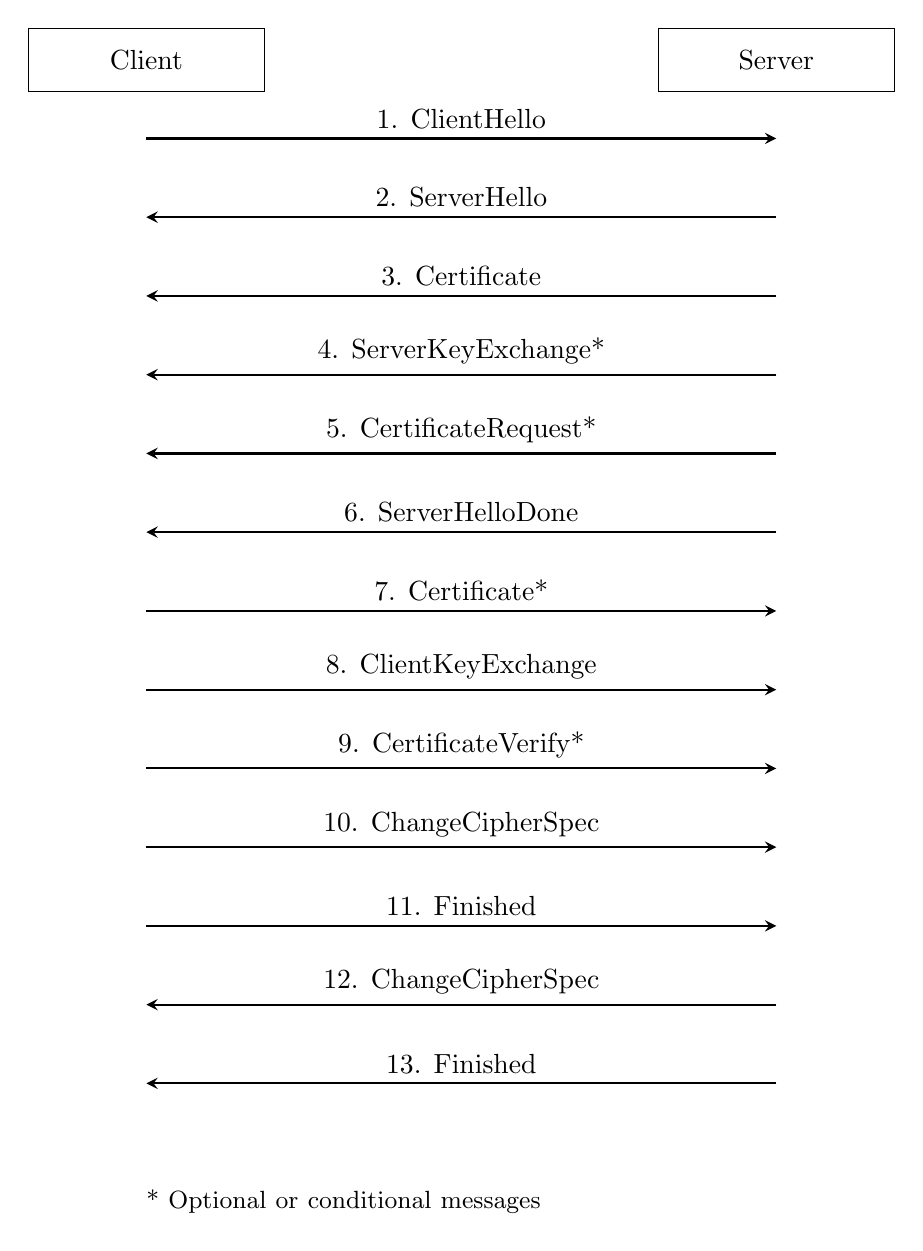
\begin{tikzpicture}[
    node distance=0.8cm,
    message/.style={->,>=stealth,thick},
    box/.style={rectangle,draw,minimum width=3cm,minimum height=0.8cm}
]

% Client and Server nodes
\node[box] (client) at (0,0) {Client};
\node[box] (server) at (8,0) {Server};

% Messages
\draw[message] (0,-1) -- node[above,sloped] {1. ClientHello} (8,-1);
\draw[message] (8,-2) -- node[above,sloped] {2. ServerHello} (0,-2);
\draw[message] (8,-3) -- node[above,sloped] {3. Certificate} (0,-3);
\draw[message] (8,-4) -- node[above,sloped] {4. ServerKeyExchange*} (0,-4);
\draw[message] (8,-5) -- node[above,sloped] {5. CertificateRequest*} (0,-5);
\draw[message] (8,-6) -- node[above,sloped] {6. ServerHelloDone} (0,-6);
\draw[message] (0,-7) -- node[above,sloped] {7. Certificate*} (8,-7);
\draw[message] (0,-8) -- node[above,sloped] {8. ClientKeyExchange} (8,-8);
\draw[message] (0,-9) -- node[above,sloped] {9. CertificateVerify*} (8,-9);
\draw[message] (0,-10) -- node[above,sloped] {10. ChangeCipherSpec} (8,-10);
\draw[message] (0,-11) -- node[above,sloped] {11. Finished} (8,-11);
\draw[message] (8,-12) -- node[above,sloped] {12. ChangeCipherSpec} (0,-12);
\draw[message] (8,-13) -- node[above,sloped] {13. Finished} (0,-13);

% Note
\node[text width=8cm] at (4,-14.5) {\small * Optional or conditional messages};

\end{tikzpicture}
\end{center}

\subsection{Message Descriptions}

\paragraph{1. ClientHello:} The client initiates the handshake with:

TLS version, 32-byte random, session ID, cipher suites list, compression methods, and extensions (SNI, ALPN, signature algorithms).

\paragraph{2. ServerHello:} The server selects:

TLS 1.2, 32-byte server random, session ID, single cipher suite, compression method, and extension responses.

\paragraph{3. Certificate:} X.509 certificate chain (server certificate + intermediate CAs). Client validates signature, validity, revocation status (CRL/OCSP), and hostname.

\paragraph{4. ServerKeyExchange (Optional):} For DHE/ECDHE only. Contains DH parameters ($p$, $g$, $g^a \mod p$) or ECDH public key, signed with server's private key to prevent MITM.

\paragraph{5. CertificateRequest (Optional):} If client authentication required. Specifies acceptable certificate types, trusted CAs, and signature algorithms.

\paragraph{6. ServerHelloDone:} Indicates server completed its handshake phase.

\paragraph{7. Certificate (Optional):} Client certificate chain if requested by server.

\paragraph{8. ClientKeyExchange:} Key exchange material:
\begin{itemize}
    \item \textbf{RSA}: 48-byte pre-master secret encrypted with server's public key
    \item \textbf{DHE/ECDHE}: Client's DH/ECDH public key value
\end{itemize}

\paragraph{9. CertificateVerify (Optional):} If client sent certificate, signs hash of all handshake messages with client's private key.

\subsection{Key Derivation}

Both client and server compute:

\[
\text{master\_secret} = \text{PRF}(\text{pre-master\_secret}, \text{``master secret''}, \text{ClientHello.random} + \text{ServerHello.random})
\]

\[
\text{key\_block} = \text{PRF}(\text{master\_secret}, \text{``key expansion''}, \text{ServerHello.random} + \text{ClientHello.random})
\]

From the key block: client/server write MAC keys, encryption keys, and IVs (for block ciphers).

\paragraph{10. ChangeCipherSpec (Client):} Activates encryption with newly negotiated keys.

\paragraph{11. Finished (Client):} First encrypted message. Contains verify\_data = PRF(master\_secret, "client finished", Hash(handshake\_messages)).

\paragraph{12. ChangeCipherSpec (Server):} Server activates encryption.

\paragraph{13. Finished (Server):} Encrypted message with verify\_data = PRF(master\_secret, "server finished", Hash(handshake\_messages)). Handshake complete.

The standard TLS 1.2 key exchange uses RSA (no forward secrecy), DHE ($g^{ab} \mod p$), or ECDHE ($d_s \cdot Q_c = d_c \cdot Q_s$) to establish a pre-master secret, from which the master secret is derived using PRF. Session resumption reuses cached master secrets to abbreviate the handshake.

\section{Proposal: Multi-Party Authorization in TLS}

Current TLS implementations vest complete control of the server's private key in a single entity. This creates a single point of failure and trust. We propose modifying TLS to require authorization from multiple parties before establishing a secure session.

\subsection{Proposed Approaches}

We present two approaches to enforce multi-party authorization in TLS by modifying the key derivation mechanism:

\subsubsection{Approach 1: Secret Sharing for Key Reconstruction}

\paragraph{Mechanism:} Use Shamir's Secret Sharing to split the server's private key among $n$ parties.

\paragraph{Protocol Modification:}
\begin{enumerate}
    \item \textbf{Setup Phase:}
    \begin{itemize}
        \item Server private key $sk$ is split into $n$ shares using $(t,n)$-threshold secret sharing
        \item Each party $P_i$ receives share $s_i$
        \item Public key remains in certificate
    \end{itemize}
    
    \item \textbf{Modified Handshake (RSA Key Exchange):}
    \begin{itemize}
        \item Client sends ClientHello
        \item Server sends ServerHello, Certificate, ServerHelloDone
        \item Client sends ClientKeyExchange with encrypted pre-master secret: $E_{pk}(PMS)$
        \item \textbf{NEW:} To decrypt, at least $t$ parties must cooperate:
        \begin{itemize}
            \item Each party $P_i$ contributes their share $s_i$
            \item Reconstruct complete private key: $sk = \text{Reconstruct}(s_1, s_2, \ldots, s_t)$
            \item Decrypt pre-master secret: $PMS = D_{sk}(E_{pk}(PMS))$
            \item \textbf{Critical:} Complete key $sk$ exists temporarily during decryption
        \end{itemize}
        \item Master secret derived from reconstructed PMS
    \end{itemize}
\end{enumerate}

\paragraph{Implementation Details:}

\textbf{Shamir's Secret Sharing Scheme:}

To split the server's RSA private key $sk$ into $n$ shares with threshold $t$:

\begin{enumerate}
    \item \textbf{Share Generation:}
    \begin{itemize}
        \item Choose random polynomial $f(x) = a_0 + a_1x + a_2x^2 + \cdots + a_{t-1}x^{t-1}$ where $a_0 = sk \mod p$ for large prime $p$
        \item Generate shares: $s_i = f(i) \mod p$ for $i = 1, 2, \ldots, n$
        \item Distribute share $s_i$ to party $P_i$ over secure channel
    \end{itemize}
    
    \item \textbf{Key Reconstruction (during handshake):}
    \begin{itemize}
        \item Collect $t$ shares from cooperating parties: $(i_1, s_{i_1}), (i_2, s_{i_2}), \ldots, (i_t, s_{i_t})$
        \item Use Lagrange interpolation to recover $sk = f(0)$:
        \[
        sk = \sum_{j=1}^{t} s_{i_j} \cdot \prod_{\substack{k=1\\k \neq j}}^{t} \frac{i_k}{i_k - i_j} \mod p
        \]
        \item Decrypt PMS: $PMS = sk^d \mod N$ where $d$ is RSA private exponent
        \item Securely erase reconstructed $sk$ after use
    \end{itemize}
    
    \item \textbf{Security Properties:}
    \begin{itemize}
        \item Any $t-1$ or fewer shares reveal no information about $sk$ (information-theoretic security)
        \item Shares must be refreshed periodically to prevent gradual compromise
        \item Communication between parties must be authenticated and encrypted
    \end{itemize}
\end{enumerate}

\textbf{Example with $t=3, n=5$:}

Suppose server's private key $sk = 12345$ (simplified), prime $p = 15485863$:

\begin{itemize}
    \item Random polynomial: $f(x) = 12345 + 7891x + 2468x^2 \mod p$
    \item Generate shares:
    \begin{align*}
        s_1 &= f(1) = 12345 + 7891 + 2468 = 22704 \mod p \\
        s_2 &= f(2) = 12345 + 15782 + 9872 = 37999 \mod p \\
        s_3 &= f(3) = 12345 + 23673 + 22212 = 58230 \mod p \\
        s_4 &= f(4) = 12345 + 31564 + 39488 = 83397 \mod p \\
        s_5 &= f(5) = 12345 + 39455 + 61700 = 113500 \mod p
    \end{align*}
    \item Any 3 shares can reconstruct $sk$, but 2 or fewer cannot
    \item To decrypt during handshake: collect shares from any 3 parties, reconstruct $sk$, decrypt PMS
\end{itemize}

\subsubsection{Approach 2: Threshold Decryption of Master Secret}

\paragraph{Mechanism:} Use threshold encryption (e.g., ElGamal, Paillier) where decryption inherently requires multiple parties without ever reconstructing the private key.

\paragraph{Protocol Modification:}
\begin{enumerate}
    \item \textbf{Setup Phase:}
    \begin{itemize}
        \item Generate threshold public key $pk$ through distributed key generation (DKG)
        \item Each party $P_i$ holds private key share $sk_i$
        \item $pk$ cannot decrypt without $t$ parties cooperating
        \item Certificate contains threshold public key $pk$
    \end{itemize}
    
    \item \textbf{Modified Handshake:}
    \begin{itemize}
        \item Standard ClientHello, ServerHello, Certificate exchange
        \item Client sends ClientKeyExchange: $C = E_{pk}(PMS)$
        \item \textbf{NEW:} Threshold decryption without key reconstruction:
        \begin{itemize}
            \item Each party $P_i$ computes decryption share: $d_i = D_{sk_i}(C)$
            \item Shares include zero-knowledge proofs of correctness
            \item Combiner aggregates shares: $PMS = \text{ThresholdDecrypt}(d_1, \ldots, d_t, C)$
            \item \textbf{Key property:} Individual $sk_i$ never combined; PMS computed from shares
        \end{itemize}
        \item Master secret derived: $MS = \text{PRF}(PMS, \text{label}, \text{randoms})$
        \item Session keys derived from master secret
    \end{itemize}
    
    \item \textbf{Verification:}
    \begin{itemize}
        \item Each party can publish proof that decryption share is correctly computed
        \item Client or auditor verifies proofs before accepting PMS
        \item Prevents malicious parties from contributing invalid shares
    \end{itemize}
\end{enumerate}

\paragraph{Advantages:}
\begin{itemize}
    \item Private key never exists in complete form (stronger security model)
    \item Individual compromise of $< t$ parties reveals nothing
    \item Zero-knowledge proofs ensure correctness
    \item Can support proactive secret sharing (refresh shares periodically)
    \item Natural fit for distributed systems and multi-organizational trust
\end{itemize}

\paragraph{Disadvantages:}
\begin{itemize}
    \item Requires changes to TLS cipher suite specifications
    \item More complex DKG setup protocol
    \item Computational overhead for threshold operations
\end{itemize}

\end{document}
